\chapter{Relational Algebra}

\section{Relational Structures}

\subsection{Preliminaries}
\begin{definitionbox}{Schema}
  A description of the database structure.
  \begin{itemize}
    \item {Tables, names and types.
          \begin{minted}{sql}
CREATE TABLE foo (bing INTEGER, zog TEXT, bar INTEGER); 
            \end{minted}
          }
    \item {Integrity constraints (foreign keys, nullability, uniqueness etc)
          \begin{minted}{sql}
ALTER TABLE foo ADD CONSTRAINT foo_key UNIQUE(bing);
                \end{minted}
          }
  \end{itemize}
\end{definitionbox}

\begin{examplebox}{Foreign Key}
  What is a foreign key constraint? Is it \textit{like a pointer}?
  \tcblower
  \begin{center}
    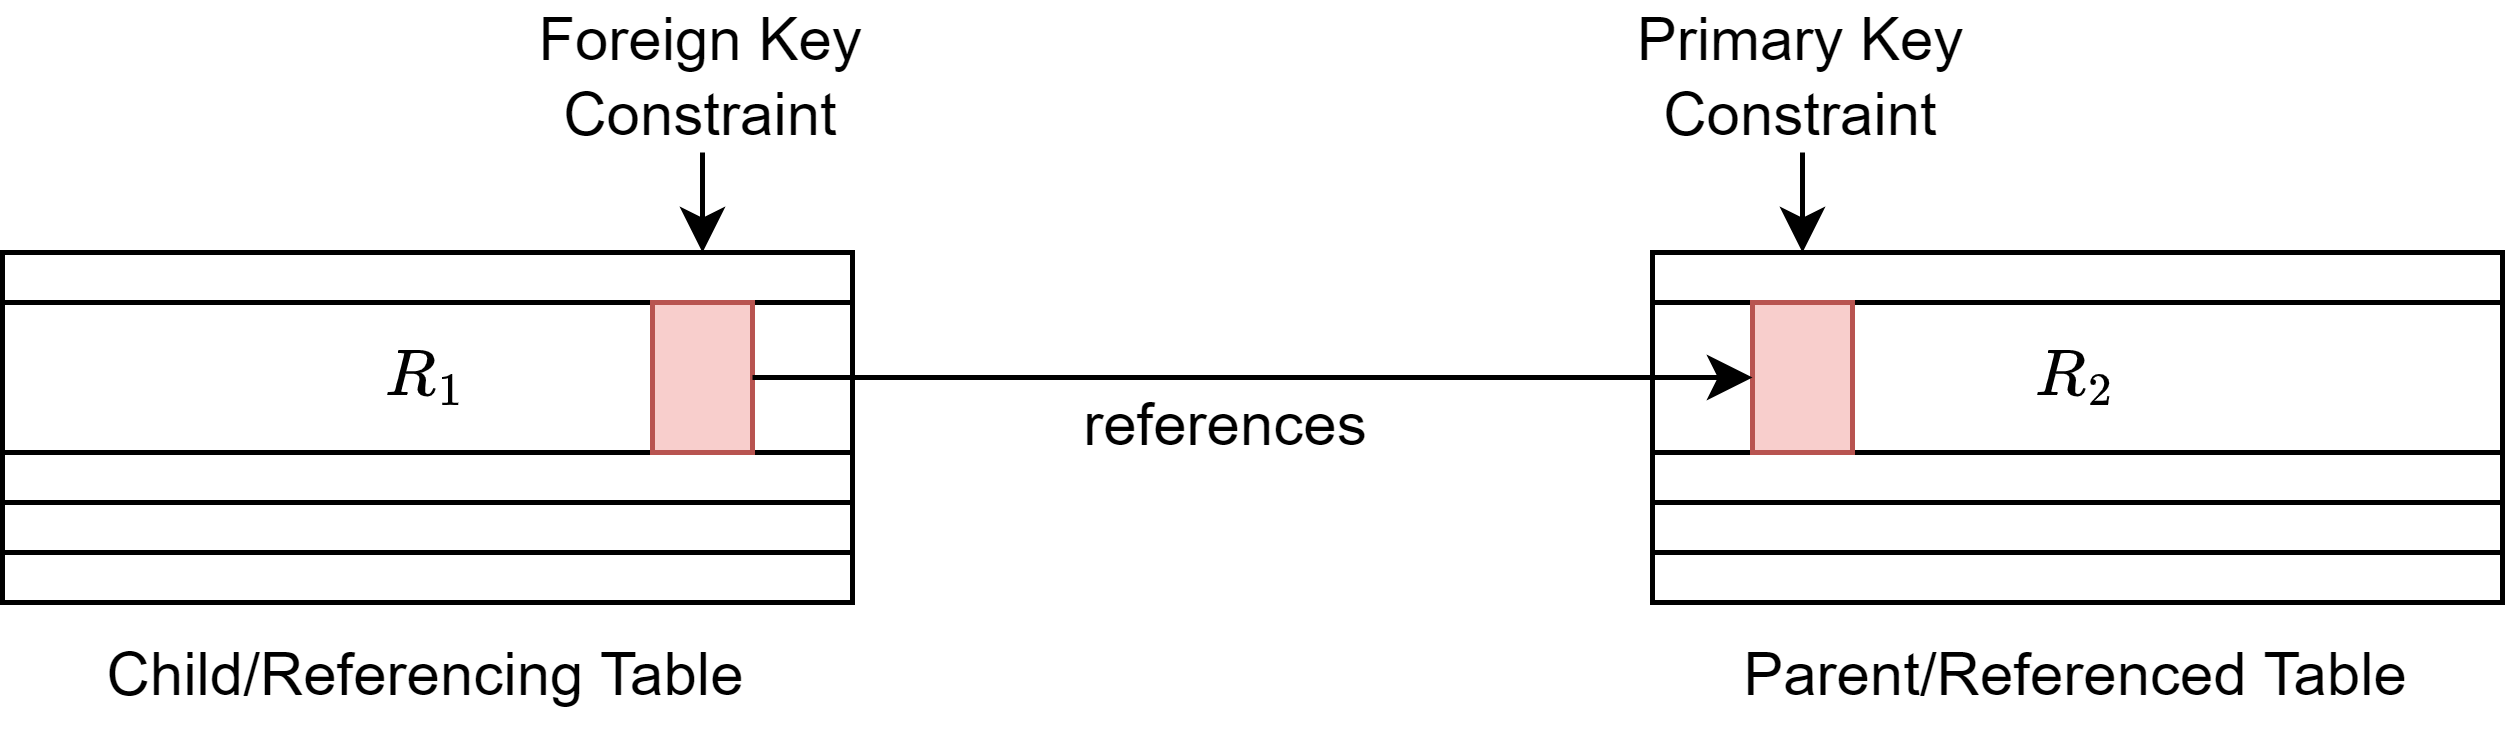
\includegraphics[width=.7\textwidth]{relational_algebra/images/example_answer_foreign_key.drawio.png}
  \end{center}
  It adds the invariant that there is a record referenced by the foreign key.
  \\
  \\ It is not really \textit{like a pointer} as:
  \begin{itemize}
    \item Not in memory (e.g on disk, different machine etc)
    \item No constant lookup (a pointer can be dereferenced in constant time, but looking up a key in a table is not necessarily)
  \end{itemize}
\end{examplebox}
\noindent
Data structures used include:
\begin{center}
  \begin{tabular}{l p{.8\textwidth}}
    \textbf{Vector} & Ordered collection of objects (same type)              \\
    \textbf{Tuple}  & Ordered collection of objects (can be different types) \\
    \textbf{Bag}    & Unordered collection of objects (same type)            \\
    \textbf{Set}    & Unordered collection of unique objects (same type)     \\
  \end{tabular}
\end{center}

\begin{definitionbox}{Relation}
  An array representing an $n$-ary relation $R$ with the properties:
  \\ \begin{minipage}{.49\textwidth}
    \begin{enumerate}
      \setlength\itemsep{0em}
      \item Each row is an $n$-tuple of $R$
      \item Rows are unordered
      \item All rows are unique / distinct
      \item The order of columns corresponds to the ordering of the domains of $R$
      \item Each column is labelled
    \end{enumerate}
    They are almost equivalent to sets tuples (but include labels).
  \end{minipage}
  \hfill
  \begin{minipage}{.5\textwidth}
    \begin{center}
      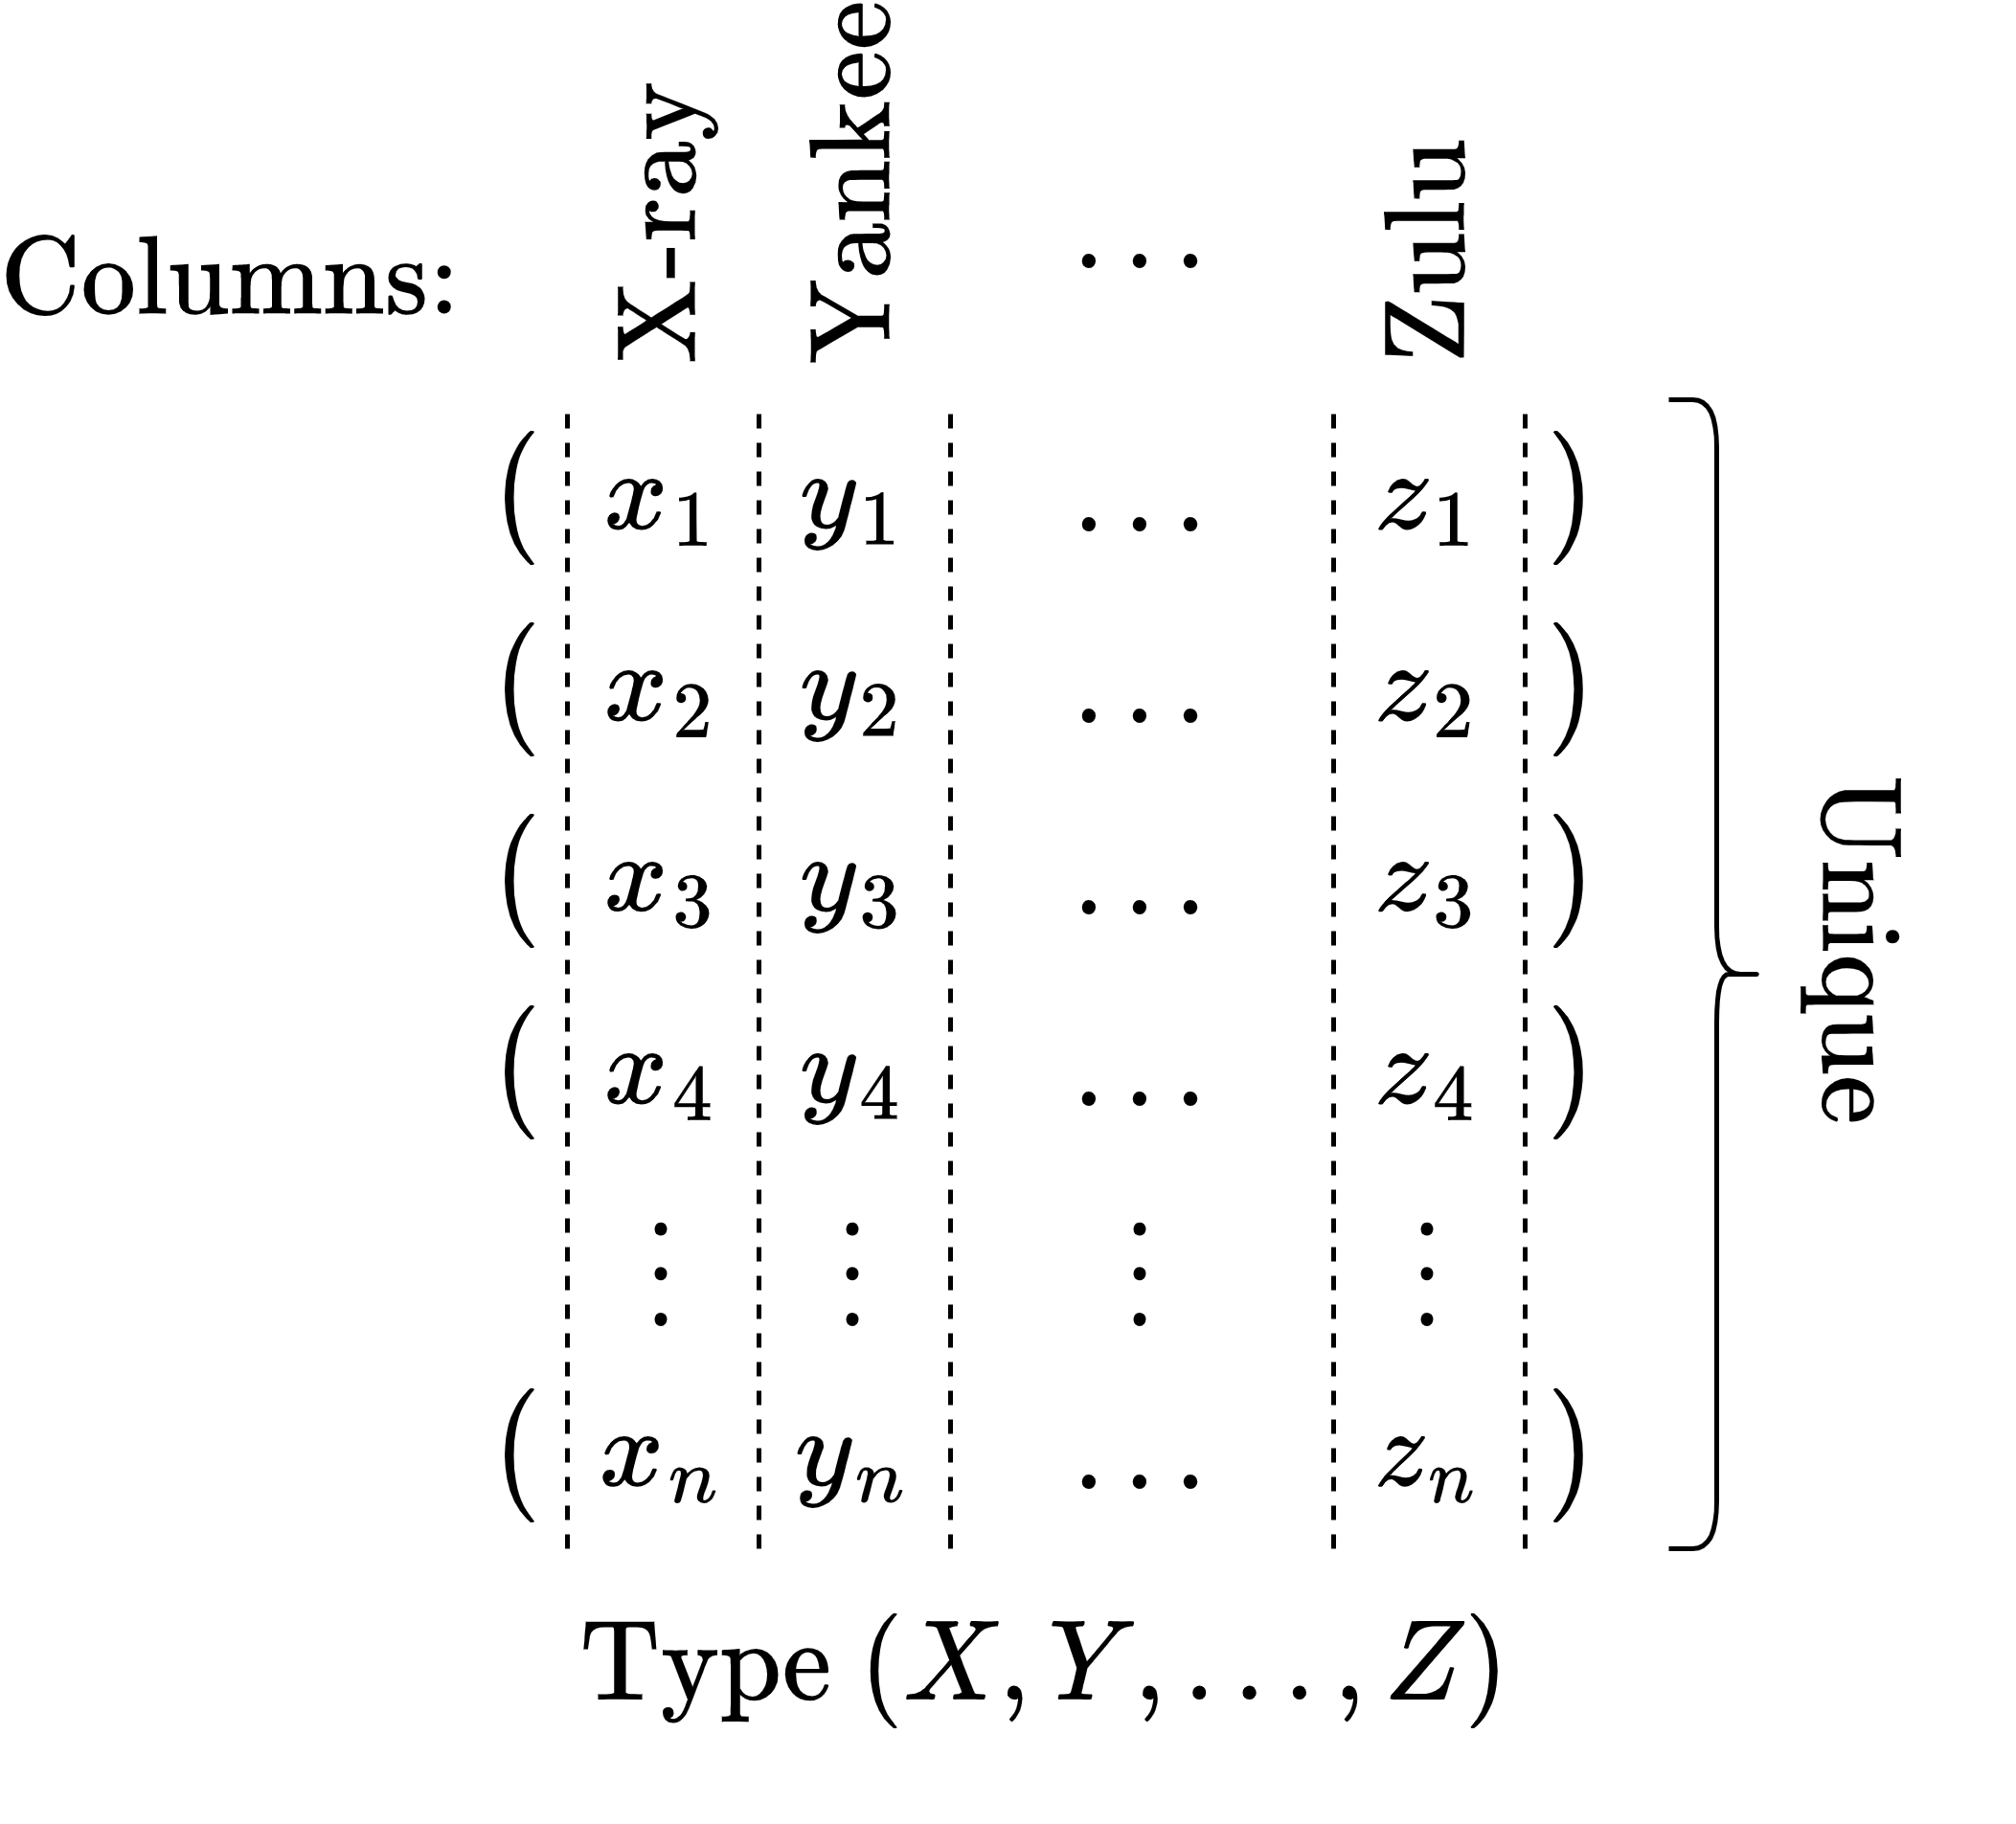
\includegraphics[width=\textwidth]{relational_algebra/images/relation.drawio.png}
    \end{center}
  \end{minipage}
\end{definitionbox}

The minimal set of operators required for the relational algebra are:
\begin{center}
  \begin{tabular}{c c c c c}
    \textbf{Project} & \textbf{Select} & \textbf{Cross/Cartesian product} & \textbf{Union} & \textbf{Difference} \\
    $\pi$            & $\sigma$        & $\times$                         & $\cup$         & $-$ or $\setminus$  \\
  \end{tabular}
\end{center}
Relational algebra is closed:
\begin{itemize}
  \item Every operator outputs a relation
  \item Operators are unary or binary
\end{itemize}

\begin{examplebox}{Query This!}
  Given the below structure, write a query to get the names of every book ordered by a current Customer in relational algebra and SQL (you may ignore differences due to bag vs set semantics).
  \begin{center}
    \begin{minipage}{.49\textwidth}
      \begin{minted}{sql}
CREATE TABLE Book (
  BookID INTEGER NOT NULL,
  Title  VARCHAR(20),
  Author VARCHAR(20),
  ISBN   VARCHAR(13)
);

CREATE TABLE OrderedItem (
  OrderID INTEGER NOT NULL,
  BookID  INTEGER NOT NULL
);

      \end{minted}
    \end{minipage} \hfill \begin{minipage}{.49\textwidth}
      \begin{minted}{sql}
CREATE TABLE Order (
  OrderID    INTEGER NOT NULL,
  CustomerID INTEGER NOT NULL,
  Price      DECIMAL(18,2)
);

-- Stores current customers
CREATE TABLE Customer (
  CustomerID      INTEGER NOT NULL,
  ShippingAddress VARCHAR(50),
  Name            VARCHAR(20) 
);
      \end{minted}
    \end{minipage}
  \end{center}
  \tcblower
  \begin{multline*}
    \Pi_{title}(\sigma_{OrderItem.BookID = Book.BookID}(\sigma_{\text{OrderedItem.OrderId = Order.OrderID}}(( \\ \sigma_{Order.CustomerID = Customer.CustomerID}(\sigma_{\text{customerID=Holger}}(Customer) \times Order)) \times OrderedItem) \times Book))
  \end{multline*}
  \begin{minted}{sql}
SELECT Book.title
FROM (
  (Customer NATURAL JOIN Order) NATURAL JOIN OrderedItem
) NATURAL JOIN Book
  \end{minted}
  Note that this will produce duplicates (bag semantics), we can remove these using a \mintinline{sql}{SELECT DISTINCT}.
\end{examplebox}

\begin{examplebox}{Unique Addresses}
  Using the previous schema create a query to get each author that has only sold to one address (can potentially ship to multiple customers at the same address)
  \tcblower
  \begin{multline*}
    \Pi_{Book.Author}(
    \sigma_{count=1}(
    \Gamma_{(Customer.ShippingAddress),(Book.Author, count)}( \\
    \Pi_{Book.Author, Customer.ShippingAddress} (
    \text{natural join}(Customer, Order, orderItem, Book)
    )
    )
    )
    )
  \end{multline*}
  Here a natural join is:
  \[\text{natural join}(R_1, R_2) \triangleq \sigma_{R_1.x_1 = R_2.x_1 \land \dots R_1.x_n = R_2.x_n} (R_1 \times R_2) \text{ where the }x\text{s are in both tables}\]
  \begin{minted}{sql}
SELECT Book.Author
FROM (
  SELECT Book.Author, Customer.ShippingAddress
  FROM ((Customer NATURAL JOIN Order) NATURAL JOIN OrderedItem) NATURAL JOIN Book
)
GROUP BY Book.Author
HAVING COUNT(*) = 1;
  \end{minted}

\end{examplebox}

\subsection{Nomenclatures}
\begin{center}
  \begin{tabular}{l p{.8\textwidth}}
    \textbf{Expression}        & A composition of operators     \\
    \textbf{Logical Plan/Plan} & An expression.                 \\
    \textbf{Cardinality}       & The number of tuples in a set. \\
  \end{tabular}
\end{center}

\section{Implementing Relational Algebra in C++}
\begin{sidenotebox}{A note on types\dots}
  Here we will express operators \& relations in the C++ types system.
  \\
  \\ In real data processing systems (and in particular databases), the schema \& types are not know at compile time (i.e do not know the types of columns, tables until they are created, amended, and operated on at runtime).
\end{sidenotebox}
\noindent
In order to implement relations we will make use of several containers from the
\href{https://en.wikipedia.org/wiki/Standard_Template_Library}{STL (standard template library)}.
\begin{minted}{cpp}
#include <set>
#include <array>
#include <string>
#include <tuple>
#include <variant>

using namespace std;
\end{minted}
We will also make use of \href{https://en.cppreference.com/w/cpp/language/parameter_pack}{\textit{variadict templates}/\textit{parameter packs}} to make our structures not only generic, but generic over $n$ types.
\begin{minted}{cpp}
template<typename... some_types>
\end{minted}
We will also create an operator to inherit from for all operator types:
\begin{minted}{cpp}
template <typename... types> struct Operator : public Relation<types...> {};
\end{minted}

\subsection{Relation}
\begin{minted}{cpp}
template <typename... types> struct Relation {
  // To allow relations to be composed, an output type is required
  using OutputType = tuple<types...>;

  set<tuple<types...>> data;              // table records
  array<string, sizeof...(types)> schema; // column names

  Relation(array<string, sizeof...(types)> schema, set<tuple<types...>> data)
      : schema(schema), data(data) {}
};
\end{minted}
\noindent
We can hence create a relation using the \mintinline{cpp}{Relation} constructor.
\begin{minted}{cpp}
Relation<string, int, int> rel(
   {"Name", "Age", "Review"},
  {{ "Jim",    33,        3}, 
   { "Jay",    23,        5}, 
   {"Mick",    34,        4}}
);
\end{minted}

\subsection{Project}
\[\Pi_{\underbrace{{a_1, \dots, a_n}}_\text{columns}}(R)\]
A unary operator returning a relation containing only the columns projected ($a_1, \dots, a_n$).
\\
\\ We can first create a projection.
\begin{minted}{cpp}
template <typename InputOperator, typename... outputTypes>
struct Project : public Operator<outputTypes...> {
  // the single input
  InputOperator input;

  // a variant is a type safe union. It is either a function on rows, or a 
  // mapping of columns 
  variant<function<tuple<outputTypes...>(typename InputOperator::OutputType)>,
          set<pair<string, string>>>
      projections;

  // Constructor for function application
  Project(InputOperator input,
          function<tuple<outputTypes...>(typename InputOperator::OutputType)>
              projections)
      : input(input), projections(projections) {}

  // Constructor for column mapping
  Project(InputOperator input, set<pair<string, string>> projections)
      : input(input), projections(projections) {}
};
\end{minted}

\begin{sidenotebox}{SQL vs RA}
  The default SQL projection does not return a set but rather a multiset / bag. In order to remove duplicates the \mintinline{sql}{DISTINCT} keyword must be used.
\end{sidenotebox}

\subsection{Select}
\[\sigma_{\text{predicate}}(R) \]
Produce a new relation of input tuples satisfying the predicate. Here we narrow this to a condition.

\begin{minted}{cpp}
enum class Comparator { less, lessEqual, equal, greaterEqual, greater };

struct Column {
  string name;

  // user must explicitly set string as a column (less chance of mistake)
  explicit Column(string name) : name(name) {}
  Column() = delete;
};

// type alias for comparable values
using Value = variant<string, int, float>;

struct Condition {
  Comparator compare;

  Column leftHandSide;
  variant<Column, Value> rightHandSide;

  Condition(Column leftHandSide, Comparator compare,
            variant<Column, Value> rightHandSide)
      : leftHandSide(leftHandSide), compare(compare),
        rightHandSide(rightHandSide) {}
};

template <typename InputOperator> 
struct Select : public Operator<typename InputOperator::OutputType> {
  InputOperator input;
  Condition condition;

  Select(InputOperator input, Condition condition) : input(input), condition(condition) {};
};
\end{minted}

\begin{sidenotebox}{Enums vs Enum classes}
  \begin{center}
    \begin{tabular}{p{.45\textwidth} p{.45\textwidth}}
      \centerline{\mintinline{cpp}{enum class}}  & \centerline{\mintinline{cpp}{enum}}            \\
      Enumerations are in the scope of the class & Enumerations are in the same scope as the enum \\
      No implicit conversions.                   & Implicit conversions to integers.              \\
    \end{tabular}
  \end{center}
  Enum classes are generally preferred over enums due to the above differences.
\end{sidenotebox}

\subsection{Cross Product / Cartesian}
\[R_1 \times R_2\]
Creates a new schema concatenating the columns and with the cartesian product of records.
\\
\\ In order to concatenate the types of the product relations we create \mintinline{cpp}{Concat<left types..., right types...>}.
\begin{minted}{cpp}
// declare the empty struct used to bind types
template <typename, typename> struct ConcatStruct;

// Table both types, create a type alias within the scope of ConcatStruct that 
// concatenates the lists of types 
template <typename... First, typename... Second>
struct ConcatStruct<std::tuple<First...>, std::tuple<Second...>> {
  using type = std::tuple<First..., Second...>;
};

// expose the type alias outside of the scope of concatStruct 
template <typename L, typename R>
using Concat = typename ConcatStruct<L, R>::type;
\end{minted}
\begin{sidenotebox}{Template Magic}
  If you are interested in how this works, see \href{https://en.cppreference.com/w/cpp/language/template_specialization}{cppreference - template specialisation}.
\end{sidenotebox}

\begin{minted}{cpp}
// Concat<> is used to concatenate the types from both input relations to 
// produce a new schema
template <typename LeftInputOperator, typename RightInputOperator>
struct CrossProduct
    : public Operator<Concat<typename LeftInputOperator::OutputType,
                             typename RightInputOperator::OutputType>> {
  // The input relations
  LeftInputOperator leftInput;
  RightInputOperator rightInput;

  CrossProduct(LeftInputOperator leftInput, RightInputOperator rightInput)
      : leftInput(leftInput), rightInput(rightInput){};
};
\end{minted}

\subsection{Union}
\[R_1 \cup R_2\]
The union of both relations, duplicates are eliminated.
\begin{minted}{cpp}
template <typename LeftInputOperator, typename RightInputOperator>
struct Union : public Operator<typename LeftInputOperator::outputType> {
  
  LeftInputOperator leftInput;
  RightInputOperator rightInput;

  Union(LeftInputOperator leftInput, RightInputOperator rightInput)
      : leftInput(leftInput), rightInput(rightInput){};
};
\end{minted}

\subsection{Difference}
\[R_1 - R_2\]
Get the set difference between two relations.

\begin{minted}{cpp}
template <typename LeftInputOperator, typename RightInputOperator>
struct Difference : public Operator<typename LeftInputOperator::outputType> {

  LeftInputOperator leftInput;
  RightInputOperator rightInput;
  
  Difference(LeftInputOperator leftInput, RightInputOperator rightInput)
      : leftInput(leftInput), rightInput(rightInput){};
};
\end{minted}

\subsection{Group Aggregation}
\[\Gamma_{(\text{grouping attributes}),(\text{aggregates})}(R)\]
\begin{itemize}
  \item Records are grouped by equality on the \textit{grouping attributes}
  \item A set of \textit{aggregates} are produced (either a grouping attribute, the result of an aggregate function, or output attribute (e.g constants))
\end{itemize}

This is implemented by \mintinline{sql}{GROUP BY} in SQL:
\begin{minted}{sql}
SELECT -- aggregates
FROM -- R
GROUP BY -- grouping attributes
\end{minted}

\begin{minted}{cpp}
// Aggregate functions to apply, 'agg' is for using groupAttributes
enum class AggregationFunction { min, max, sum, avg, count, agg };

template <typename InputOperator, typename... Output>
struct GroupedAggregation : public Operator<Output...> {  
  InputOperator input;

  // the attributes to group by (column names)
  set<string> groupAttributes;

  // (column, aggregate function, new column name)
  set<tuple<string, AggregationFunction, string>> aggregations;

  GroupedAggregation(
      InputOperator input, set<string> groupAttributes,
      set<tuple<string, AggregationFunction, string>> aggregations)
      : input(input), groupAttributes(groupAttributes),
        aggregations(aggregations){};
};
\end{minted}

\subsection{Top-N}
\[TopN_{(n, attribute)}(R)\]
Get the top $n$ records from a table, given the ordering of $attribute$
\\
\\ This is implemented with \mintinline{sql}{LIMIT} and \mintinline{sql}{ORDER BY} in SQL:
\begin{minted}{sql}
SELECT -- ...
FROM -- R
ORDER BY 
\end{minted}

\begin{minted}{cpp}
// note that here we include N in the type (know at compile time), we could also
// take it as a parameter constructor (known at runtime)
template <typename InputOperator, size_t N>
struct TopN : public Operator<typename InputOperator::OutputType> {
  InputOperator input;
  string predicate;

  TopN(InputOperator input, string predicate)
      : input(input), predicate(predicate){};
};
\end{minted}

\begin{sidenotebox}{Have a go!}
  The provided examples are only one way to mock up / sketch relation algebra with C++. Consider:
  \begin{itemize}
    \item Using runtime polymorphism \mintinline{cpp}{virtual} methods in derived operator classes and \mintinline{cpp}{std::variant} data types, rather than using templates.
    \item Going all-in on compile time programming with \mintinline{cpp}{constexpr}.
    \item Using \mintinline{cpp}{concept}s / \mintinline{cpp}{requires} to constrain the operator types.
  \end{itemize}
\end{sidenotebox}
